\chapter{PolyChord}
\label{chap:pc}

\epigraph{\ldots note that exploring a hard-edged likelihood-constrained domain should prove to be neither more nor less demanding than exploring a likelihood-weighted space }{\johnskilling{}}

\section{Introduction}
\label{sec:pc:introduction}
Over the past two decades, Bayesian methods have been increasingly adopted as the standard inference procedure for the rapidly increasing volume of astrophysical data.

Bayesian inference consists of {\em parameter estimation\/} and {\em model comparison}.  Parameter estimation is generally performed using Markov-Chain Monte-Carlo (MCMC) methods, such as the Metropolis-Hastings (MH) algorithm and its variants~\citep{Mackay}.  In order to perform model comparison, one must calculate the {\em evidence\/}: a high-dimensional integration of the likelihood over the prior density~\citep{Sivia}.  MH methods cannot compute this on a usable timescale, hindering the use of Bayesian model comparison in cosmology and astroparticle physics.

A contemporary methodology for computing evidences and posteriors simultaneously is provided by nested sampling~\citep{skilling2006}. This has been successfully implemented in the now widely adopted algorithm \MultiNest\,~\citep{MultiNest1,MultiNest2,MultiNest3}.  Modern cosmological likelihoods now involve a large number of parameters, with a hierarchy of speeds.  \MultiNest\ struggles with high-dimensional parameter spaces, and is unable to take advantage of this separation of speeds.  \PolyChord{} aims to address these issues, providing a means to sample high-dimensional spaces across a hierarchy of parameter speeds.

The layout of the paper is as follows:
We overview the historical implementations of nested sampling in Section~\ref{sec:pc:iso_likelihood_sampling} and provide an account of \citepos{NealSlice} slice sampling technique.
We describe the \PolyChord{} algorithm in detail in Section~\ref{sec:pc:polychord_algorithm} and demonstrate its efficacy on toy and cosmological problems in Section~\ref{sec:pc:polychord_in_action}.  
Section~\ref{sec:pc:conclusions} concludes the paper.

This paper is an extensive overview of our algorithm, which is now in use in several cosmological applications~\citep{planck2015-a24}. A briefer introduction can be found in~\cite{polychordletter}.

\PolyChord{} is available for download from the link at the end of the paper.







\section{Sampling within an iso-likelihood contour}
\label{sec:pc:iso_likelihood_sampling}

\subsection{The unit hypercube}
\label{sec:bay:unit_hypercube}
Each iteration of nested sampling requires one to sample from the prior (subject to a hard likelihood constraint). 
Typically, priors are defined in terms of simple analytic functions such as uniform or Gaussian distributions, and may be sampled using  inverse transform sampling (Appendix~\ref{sec:sm:inverse_transform}). 

Nested sampling can thus be performed in the unit $D$-dimensional hypercube. This has numerous advantages, the first being that one only needs to be able to generate uniform random variables in $[0,1]$. The second is more subtle; it is more natural to define a distance metric in the unit hypercube than in the physical space. Unit hypercube variables all have the same dimensionality: probability.



\subsection{Previous methods}
\label{sec:pc:previous_methods}
The most challenging aspect of nested sampling is drawing a new point from the prior subject to the hard likelihood constraint $\lik>\lik_i$. This may be done in a variety of ways, and distinguishes the various historical implementations.

For some problems, the iso-likelihood contour is known analytically, allowing one to construct a sampling procedure specific to that problem. This is demonstrated by~\cite{Keeton}, and can be useful for testing nested sampling's theoretical behaviour. In most cases, however, the likelihood contour is unknown a-priori, so a more numerical approach must be taken.

\cite{Mukherjee} implemented a rejection sampling (Appendix~\ref{sec:sm:rejection}) method, which was later incorporated into the widely-used~\MultiNest{} algorithm~\citep{MultiNest1,MultiNest2,MultiNest3}.
These algorithms sample by using the live points to construct a set of intersecting ellipsoids which together aim to enclose the likelihood contour, and then performs rejection sampling within the ellipsoids.
 Whilst being an excellent algorithm for modest numbers of parameters, any rejection sampling algorithm has an exponential scaling with dimensionality that eventually emerges.

An alternative approach (the one initially envisaged by Skilling) is to sample with the hard likelihood constraint using a Markov-Chain based procedure. One makes several steps according to some proposal distribution until one is satisfied an independent sample is produced. This has significant advantages over a rejection-based approach, the most obvious being that the scaling with dimensionality is polynomial rather than exponential. In rejection sampling, points are drawn until one is found within the likelihood contour (often with extremely low efficiency). Using a Markov-chain approach however, (correlated) points are continually generated within the contour, until one is happy that a sample independent from the initial seed has been generated. These ``intra-chain points'' which we term {\em phantom points\/} have the potential to provide a great deal more information.

A traditional Metropolis-Hastings (MH) or Gibbs sampling approach may be utilised, but in general such algorithms are ill-suited to sampling from a hard likelihood constraint without a significant amount of tuning of a proposal matrix. This is examined in section 6 of~\cite{MultiNest1}.

Galilean (Hamiltonian) sampling~\citep{GalileanNestedSampling,Betancourt2011} improves upon the traditional MH sampler by using proposal points generated by reflecting off iso-likelihood contours. This however requires gradients to be calculated, and can become inefficient if the step size is chosen incorrectly, or if the contour has a shape which is difficult to `step back into'

Diffusive nested sampling~\citep{DiffusiveNestedSampling} is an alternative and promising variation on~\citepos{skilling2006} algorithm, which utilises MCMC to explore a mixture of nested probability distributions. Since it is MCMC based, it scales well with dimensionality. In addition, it can deal with multimodal and degenerate posteriors, unlike traditional MCMC\@. It does however have multiple tuning parameters.


\subsection{Slice sampling}
\label{sec:bay:slice_sampling}
We have found that a Markov-Chain based procedure utilising~\citepos{NealSlice} slice sampling at each step is well suited to sampling uniformly within an iso-likelihood contour.

This procedure for sampling within a likelihood bound is ideal for nested sampling. It samples uniformly with minimal information: an initial bound size $w$, and a point $x_0$ that is within the contour. In general $w$ must be chosen so that it is roughly the size of the bound, but if one overestimates it then the bounds will contract exponentially. Indeed, one may consider this as being equivalent to a prior space compression~\eqref{eqn:pc:X_full} with $\nlive=\ndims=1$. As a starting point, one may use one of the live points, which is already uniformly sampled. Since the procedure above satisfies detailed balance, this will produce a point which is also uniformly sampled within the iso-likelihood contour.

In higher dimensions,~\cite{NealSlice} suggests a variety of MCMC-like methods. The simplest of these is implemented by sampling each of the parameter directions in turn. Since each one-dimensional slice requires $\bigO{\text{a few}}$ likelihood calculations, the number of likelihood calculations required scales linearly with dimensionality, providing the region is efficiently navigated. Multi-dimensional slice sampling has many of the benefits of a traditional MH approach, and uses a proposal distribution which is much more efficient at sampling a hard likelihood constraint.

\cite{SystemsBio} have already applied this procedure to nested sampling. This works exceptionally well for cases in which the parameters are non-degenerate. However, this becomes inefficient in the case of correlated parameters, or curving degeneracies.





%Calculation of the posterior $\posterior(\theta)$ is the domain of {\em parameter estimation}, and in high dimensions is best performed by sampling the space with a Markov-Chain Monte-Carlo approach (MCMC). Examples include Metropolis-Hastings, Gibbs sampling and Slice sampling. For the most part, the evidence $\ev$ is ignored during such calculations, and one works with an unnormalised posterior ${\posterior\propto\lik\times\prior}$.





\section{The \PolyChord{} algorithm}
\label{sec:pc:polychord_algorithm}

\PolyChord{} implements several novel features compared to~\citepos{SystemsBio} slice-based nested sampling.  
It utilises slice sampling in a manner that uses the information present in the live and phantom points to deal with correlated posteriors. 
\PolyChord{} also uses a general clustering algorithm that identifies and evolves separate modes of the posterior semi-independently, and infers local evidence values.  
In addition, it has the option of implementing fast-slow parameters, which is extremely effective in its combination with \CosmoMC{}~\citep{cosmomc}. 
This is termed \CosmoChord, which may be downloaded from the link at the end of the paper.

 The algorithm is written in \FORTRAN{} and parallelised using \openMPI{}.  It is optimised for the case where the dominant cost is the generation of a new live point.  This is frequently the case in astrophysical applications, either due to high dimensionality, or to costly likelihood evaluation.  

%
\begin{figure}[tp]
  \centerline{%
    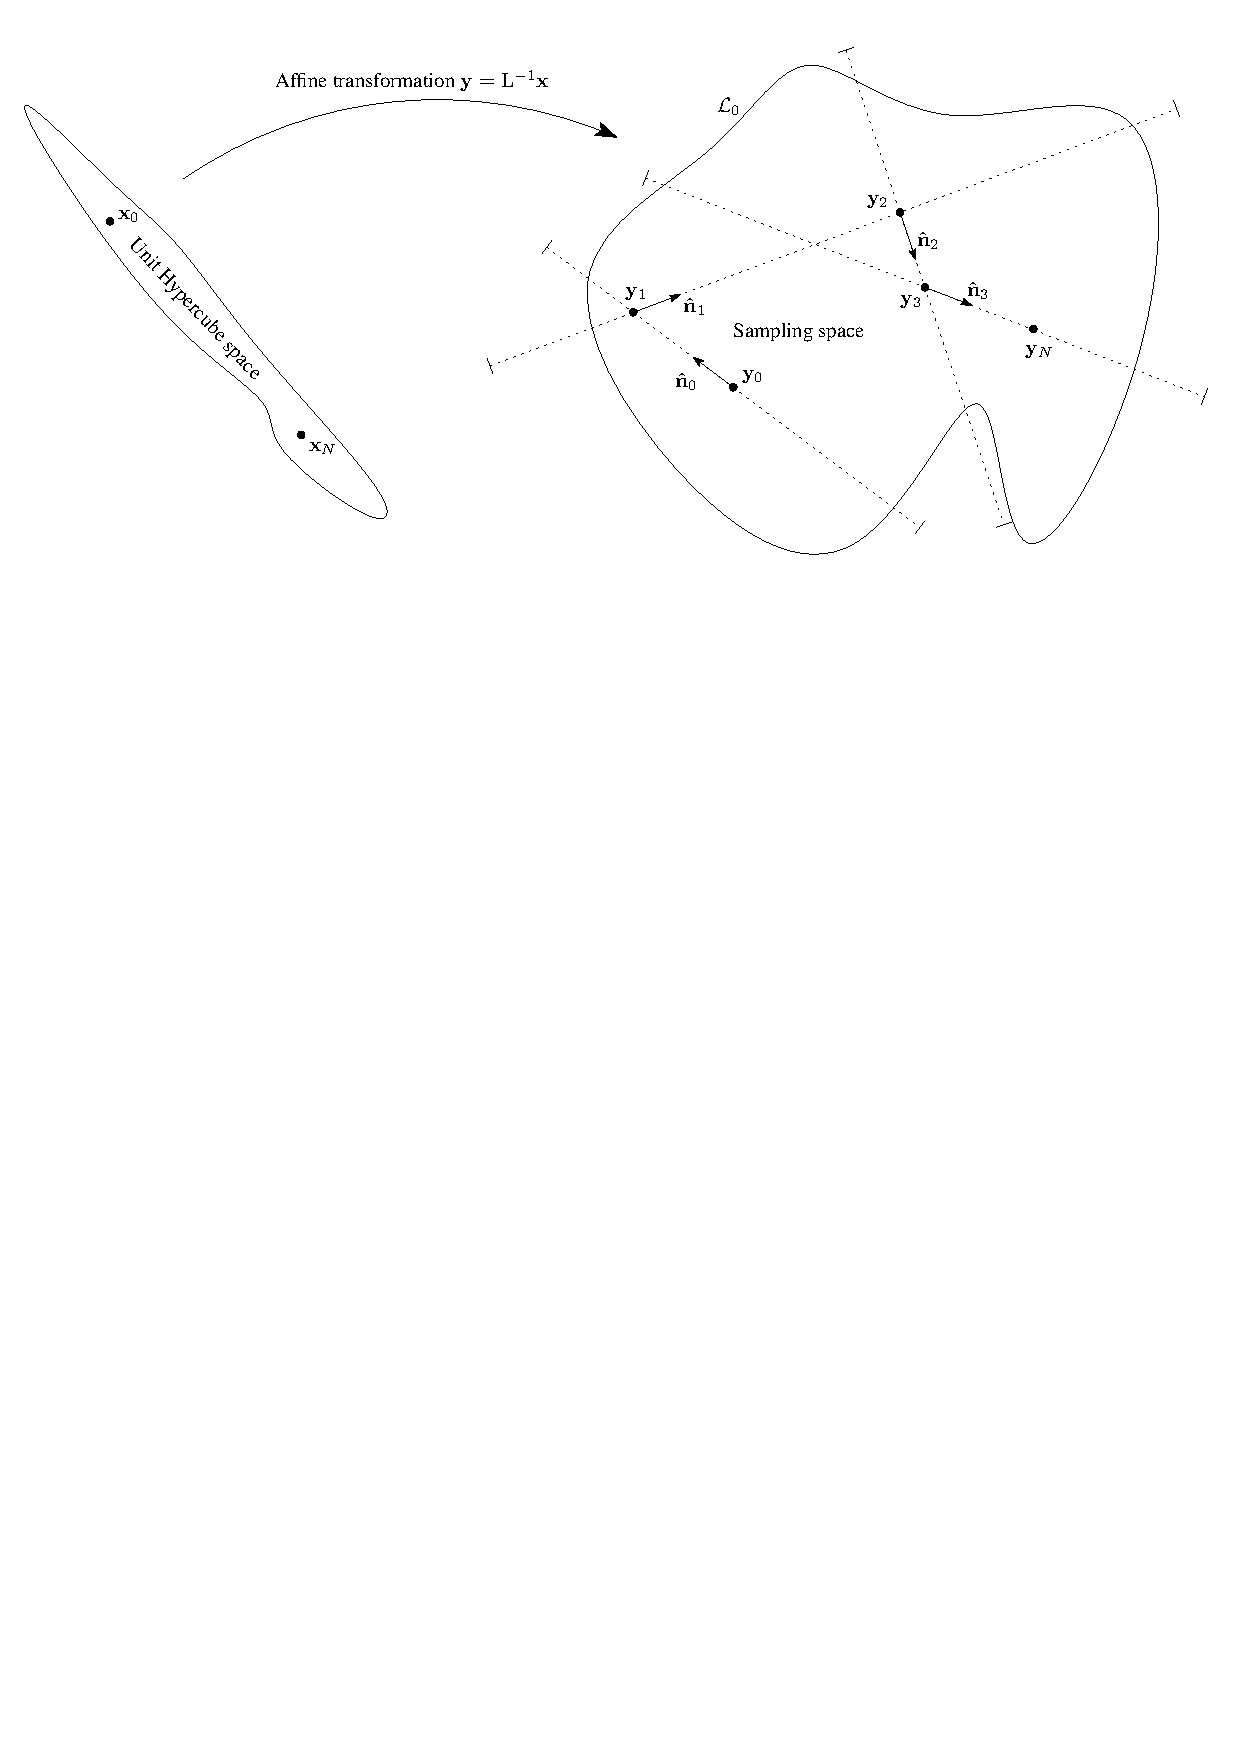
\includegraphics[width=\textwidth]{chapters/polychord/figures/contour}
}
\caption{%
  Slice sampling in $D$ dimensions. 
  We begin by ``whitening'' the unit hypercube by making a linear transformation which turns a degenerate contour into one with dimensions $\bigO{1}$ in all directions. 
  This is a linear skew transformation defined by the inverse of the Cholesky decomposition of the live points' covariance matrix. 
  We term this whitened space the {\em sampling space}. 
  Starting from a randomly chosen live point $\bx{0}$, we pick a random direction and perform one-dimensional slice sampling in that direction (Appendix~\protect\ref{sec:sm:slice}), using $w=1$ in the sampling space. 
  This generates a new point $\bx{1}$ in $\bigO{\text{a few}}$ likelihood evaluations. 
  This process is repeated $\bigO{\ndims}$ times to generate a new uniformly sampled point $\bx{N}$ which is decorrelated from $\bx{0}$.\label{fig:pc:Nd_slice}
}
\end{figure}
%

\subsection{Multi-dimensional slice sampling}
\label{sec:pc:multi_slice}
At each iteration $i$ of nested sampling, we generate a new randomly sampled point within the iso-likelihood contour $\lik_i$ by our variant of $D$-dimensional slice sampling.
Slice sampling is performed in the unit hypercube with hypercube co\"{o}rdinates denoted in bold ($\bxx$).

At each iteration $i$ of the nested sampling algorithm, one of the live points is chosen at random as a start point for a new chain with hypercube co\"{o}rdinate $\bx{0}$. We then make a one-dimensional slice sampling step (Appendix~\protect\ref{sec:sm:slice}) with initial width $w$ in a random direction $\nhat{0}$ chosen from a probability distribution $\Prob{\nhatx}$. This generates a new point $\bx{1}$ which is uniformly sampled in the unit hypercube, but is correlated to $\bx{0}$. This process is repeated $\nrepeats$ times, with $\bx{j-1}$ forming the start point for a slice along $\nhat{j-1}$ to produce $\bx{j}$. This procedure is illustrated in the right hand half of Figure~\ref{fig:pc:Nd_slice}.

Since the probability of drawing $\bx{j}$ from $\bx{j-1}$ is the same as the probability of drawing $\bx{j-1}$ from $\bx{j}$, this procedure satisfies detailed balance. Thus, the resulting chain will ergodically be uniformly distributed within the iso-likelihood contour. This also applies to multi-modal posteriors, with the chance of jumping out a mode being equal to the chance of jumping back in.

The length of the chain $\nrepeats$ should be large enough so that the final point of the chain is decorrelated from the start point. 
This final point may now be considered to be a new uniformly sampled point from the prior distribution subject to the hard likelihood constraint. The intermediate points are saved and stored as phantom points. Whilst phantom points are correlated, they are useful in providing additional information and posterior points.

There are several elements of this which are left undetermined, namely the probability distribution $\Prob{\nhatx}$, the initial width $w$, and the chain length $\nrepeats$. These issues are addressed in the next section.


\subsection{Contour whitening}
\label{sec:pc:cont_white}
In order to determine an optimal $\Prob{\nhatx}$ and $w$, an algorithm will need some knowledge of the contour in which the chain is progressing. This information can be supplied by the set of live and phantom points which are already uniformly distributed within the contour. We use the sample covariance matrix of the live and phantom points as a proxy for the size and shape of the contour.

Uniformly sampled points remain uniformly sampled under an affine transformation. The covariance matrix is used to construct an affine transformation which ``whitens'' the contour. Sampling is then performed in this whitened space, which we term the {\em sampling space}.
In the sampling space, the contour has size $\bigO{1}$ in every direction. This means that one may choose the initial step size as $w=1$.

To transform from $\bxx$ in the unit hypercube to $\byy$ in the sampling space we use the relation:
\begin{equation}
  \mathrm{L}^{-1}\bxx =  \byy,
  \label{eqn:pc:cholesky}
\end{equation}
where $\mathrm{L}$ is the Cholesky decomposition of the covariance matrix $\Sigma = \mathrm{L} \mathrm{L}^{T}$.
This is illustrated further in Figure~\ref{fig:pc:Nd_slice}.

Working in the sampling space our choice of $\Prob{\nhatx}$ is inspired by the default choice of \CosmoMC{}~\citep{LewisFastSlow}. Here, a randomly oriented orthonormal basis is chosen, and these directions are chosen in a random order. Once a basis is exhausted, a new basis is chosen. This approach satisfies detailed balance, and mixes rapidly.

The choice of $\nrepeats$ is slightly harder to justify. We find that for distributions with roughly convex contours $\nrepeats\bigO{\ndims}$ is sufficient, with the constant of proportionality being $2$---$6$. For more complicated contour shapes, one may require much larger values of $\nrepeats$. 

This procedure has the advantage of being dynamically adaptive, and requires no tuning parameters. However, this ``whitening'' process is ineffective for pronounced curving degeneracies. This will be discussed in detail in Section~\ref{sec:pc:gaussian_shells}.


\subsection{Clustering}
\label{sec:pc:clustering}
Multi-modal posteriors are a challenging problem for any sampling algorithm. ``Perfect'' nested sampling (i.e.\ the entire prior volume enclosed by the iso-likelihood contour is sampled uniformly) in theory solves multi-modal problems as easily as uni-modal ones. In practice however, there are two issues.

First, one is limited by the resolution of the live points. If a given mode is not populated by enough live points, it runs the risk of ``dying out''. Indeed, a mode may be entirely missed if the density of live points is too low. In many cases, this problem can be alleviated by increasing the number of live points.

Second, and more importantly for \PolyChord{}, the sampling procedure may not be appropriate for multi-modal problems. We ``whiten'' the unit hypercube using the covariance matrix of live points. For far-separated modes, the covariance matrix will not approximate the dimensions of the contours, but instead falsely indicate a high degree of correlation.  It is therefore essential for our purposes to have \PolyChord{} recognise and treat modes appropriately.


This methodology splits into two distinct parts:
  (i) recognising that clusters are there, and
  (ii) evolving the clusters semi-independently.

\subsubsection{Cluster recognition}
\label{sec:pc:clustering_recognition}
Any cluster recognition algorithm can be substituted at this point.  One must take care that this is not run too often, or one runs the risk of adding a large overhead to the calculation.  In practice, checking for clustering every $\bigO{\nlive}$ iterations is sufficient, since the prior will have only compressed by a factor $e$.  We encourage users of \PolyChord{} to experiment with their own preferred cluster recognition, in addition to that provided and described below. 

It should be noted that the live points of nested sampling are amenable to most cluster recognition algorithms for two reasons.  First, all clusters should have the same density of live points in the unit hypercube.  Second, there is no noise (i.e.\ outside of the likelihood contour there will be no live points). Many clustering algorithms struggle when either of these two conditions is not satisfied.

We therefore choose a relatively simple variant of the $k$-nearest neighbours algorithm to perform cluster recognition.  If two points are within one another's $k$-nearest neighbours, then these two points belong to the same cluster.  We iterate $k$ from $2$ upwards until the clustering becomes stable (the cluster decomposition does not change from one $k$ to the next).  If sub-clusters are identified, then this process is repeated on the new sub-clusters.

\subsubsection{Cluster evolution}
\label{sec:pc:clustering_evolution}
An important novel feature comes from what one does once clusters are identified. 

First, when spawning from an existing live point, the whitening procedure is now defined by the covariance matrix of the live points within that cluster. This solves the issue detailed above.

Second, by choosing a random initial live point as a seed, \PolyChord{} would na\"{\i}vely spawn live points into a mode with a probability proportional to the number of live points in that mode. In fact, what it should be doing is to spawn in proportion to the volume fraction of that mode. In general, these will be approximately the same, but numerical experiments show that the difference between these two ratios exhibits random-walk like behaviour, leading to biases in evidence calculations, or worse, cluster death. 

Instead, we keep track of an estimate of the volume in the same manner as equation~\eqref{eqn:pc:X_full}, and choose the mode to spawn into in proportion to that estimate. Further, one may track the errors in this estimate, which contribute to the overall evidence error. This methodology is documented fully in Section~\ref{sec:ens:evidences_clusters}.

Thus, the point to be killed off is still the global lowest-likelihood point, but we control the spawning of the new live point into clusters by using our estimates of the volumes of each cluster. We call this `semi-independent', because it retains global information, whilst still treating the clusters as separate entities. 

When spawning within a cluster, we determine the cluster assignment of the new point by which cluster it is nearest to. It does not matter if clusters are identified too soon; the evidence calculation will remain consistent.

In addition to keeping track of local volumes, we may keep track of local evidences. At the moment of splitting, the existing evidence in the initial cluster is partitioned between the new sub-clusters. Upon algorithm completion, one is left with an estimate of the proportion of the evidence contained within each cluster, and thus a measure of the importance of the various modes. By partitioning the local evidences at cluster recognition, the local evidences will sum to give the total evidences, to within the error on our inference.


\subsection{Parallelisation}
\label{sec:pc:parallelisation}
\PolyChord{} is parallelised by \openMPI{} using a master-slave structure.  One master process takes the job of organising all of the live points, whilst the remaining ${\nprocs-1}$ ``slave'' processes take the job of finding new live points. This layout is optimised for the case where the dominant cost is the generation of a new live point due to the calculation of relatively expensive likelihoods.

When a new live point is required, the master process sends a random live point and the Cholesky decomposition to a waiting slave.  The slave then, after some work, signals to the master that it is ready and returns a new live point and the intra-chain points to the master.

A point generated from an iso-likelihood contour $\lik_i$ is usable as a new live point for an iso-likelihood contour $\lik_j>\lik_i$, providing it is within both contours.  One may keep slaves continuously active, and discard any points returned which are not usable.  The probability of discarding a point is proportional to the volume ratio of the two contours, so if too many slaves are used, then most will be discarded.  The parallelisation goes as:
\begin{equation}
  \text{Speedup}(\nprocs) = \nlive\log\left[ 1 + \frac{\nprocs}{\nlive} \right],
  \label{eqn:pc:parallel}
\end{equation}
and is illustrated in Figure~\ref{fig:pc:parallel}. 
As a rule, \PolyChord{} parallelises well for $\nprocs<\nlive$, but from exhibits a law of diminishing returns. In practice, $\nprocs = \nlive/5$ yields $\sim90\%$ parallelisation efficiency, and
since the number of live points is typically $\sim500$, this is more than sufficient for currently available \openMPI{} architectures, and certainly superior to the parallelisation of the standard Metropolis-Hastings algorithm.
%
\begin{figure}[tp]
  \centering
  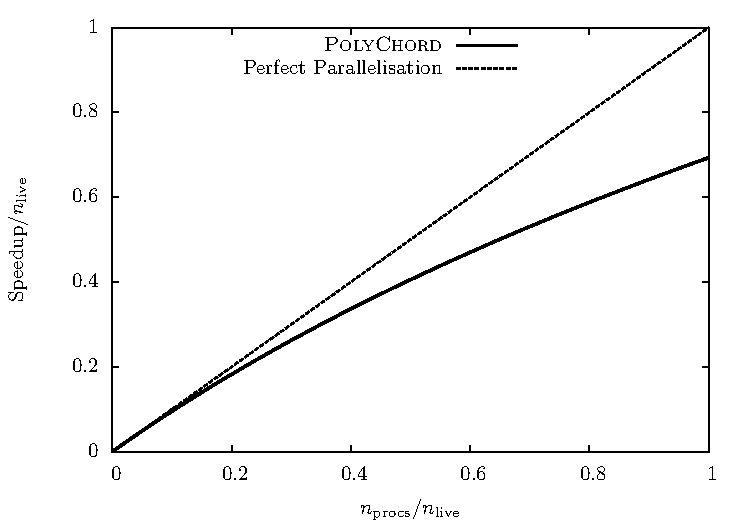
\includegraphics[width=\columnwidth]{chapters/polychord/figures/parallel}
  \caption{%
Parallelisation of \PolyChord{}. 
The algorithm parallelises nearly linearly, providing that $\nprocs<\nlive$. For most astronomical applications this is more than sufficient.\label{fig:pc:parallel}}
\end{figure}
%
\subsection{Posterior bulking}
\label{sec:pc:posterior_bulking}
In addition to lending information on the scale and shape of a contour, phantom points can also be used as posterior samples. Correlations between samples are unimportant for the purposes of parameter estimation, providing one has enough to be well mixed. We may thus use the importance weighting detailed in~\eqref{eqn:bay:posterior_weight} with $w_i$ being set to the volume of the live-point shell which they occupy.

For high-dimensional cosmological applications, this results in a very large number ($\gg$GB) of posterior samples being produced, so \PolyChord{} thins these samples. From a user's perspective, one supplies a parameter which determines the fraction of phantom points to keep.

\subsection{Fast-slow parameters and \CosmoChord}
\label{sec:pc:fast_slow}

In cosmological applications, likelihoods can exhibit a hierarchy of parameters in terms of calculation speed~\citep{LewisFastSlow}. Consequently, a likelihood may be quickly recalculated if one changes only a certain subset of the parameters. For \PolyChord{} it is very easy to exploit such a hierarchy. Our transformation to the sampling space is laid out so that if parameters are ordered from slow to fast, then this hierarchy is automatically exploited: a Cholesky decomposition, being a upper-triangular skew transformation, mixes each parameter only with faster parameters.

From a user's perspective, \PolyChord{} does this re-ordering in the hypercube automatically when provided with details of the hierarchy.

Further to this, one may use the fast directions to extend the chain length by many orders of magnitude. This helps to ensure an even mixing of live points. \PolyChord{} automatically times likelihood calculation speeds, so the user just has to provide what fraction of time \PolyChord{} should be spending on each subset of the parameters, and the algorithm will oversample accordingly.

\subsection{Tuning parameters}
\label{sec:pc:tuning_params}

From a user's perspective, the \PolyChord{} algorithm has two tuning paramaters: $\nlive$ and $\nrepeats$, which are detailed below.

The authors believe that these tuning parameters are fairly straightforward to set in comparison to existing algorithms. More importantly, the number of tuning parameters does not scale with the dimensionality of the problem. This is in contrast to Metropolis-Hastings and Gibbs sampling, which require a proposal matrix to be supplied\footnote{Proposal matrices may be learnt during run-time. However, this learning step can take some time and may reduce the efficacy of these approaches.}.

There are also several other options controlling run time behaviour, such as the production of equally weighted posterior samples, whether or not to perform clustering and the production and use of files allowing \PolyChord{} to resume from a previous run. These are documented in the input files supplied with the code.

\subsubsection*{Resolution $\nlive$ }
This is a generic nested sampling parameter. $\nlive$ indicates the number of live points maintained throughout the algorithm. Increasing $\nlive$ causes nested sampling to contract more slowly in volume (equation~\ref{eqn:pc:X_full}), and consequently sample the space more thoroughly. Thus, it can be thought of as a resolution parameter. Run time scales $\bigO{\nlive}$

If set too low, posterior modes may be missed. Increasing $\nlive$ increases the accuracy of the inference of $\ev$, since the evidence error scales $\bigO{\nlive^{-1/2}}$. 

\subsubsection*{Reliability $\nrepeats$}
This is a \PolyChord{} specific parameter. It corresponds to the length of the slice sampling chain used to generate a new live point. Increasing this parameter decreases the correlation between live points, and hence increases the reliability of the evidence inference. Posterior estimations, however, remain accurate even in the event of low $\nrepeats$.

Setting this too low can result in correlation between live points, and unreliable evidence estimates. Typically, setting this $\bigO{3\times\ndims}$ is sufficient, but for curving degeneracies one may need significantly longer chains. Run time scales $\bigO{\nrepeats}$. 

The total number of live and phantom points ${\nlive\times\nrepeats}$ should be large enough that reliable covariance matrices can be calculated. Other than this, the two tuning parameters have independent effects on the algorithm. 

In general, $\nrepeats$ should be scaled linearly with dimensionality $D$, since one must decorrelate in $D$ independent directions. For typical likelihoods, the logarithmic volume compression from prior to posterior will scale as $D$. Finally, to keep evidence estimation error constant, the number of live points must be scaled with $D$. These three effects together mean that \PolyChord{} has a theoretical run time scaling $\bigO{D^3}$.

\section{\PolyChord{} in action}
\label{sec:pc:polychord_in_action}
We aim to showcase \PolyChord{} as both a high-dimensional evidence calculator, and multi-modal posterior sampler. We begin by comparing its dimensionality scaling with \MultiNest{}. We then demonstrate its clustering capabilities in high dimensions, and on difficult clustering problems. \PolyChord{} is shown to perform well on moderately pronounced curving degeneracies, and its implementation in \CosmoMC{} is discussed.

\subsection{High-dimensional evidences}
\label{sec:pc:hi_ev}

As an example of the strength of \PolyChord{} as a high-dimensional evidence estimator, we compare it to \MultiNest{} on a Gaussian likelihood in $D$ dimensions.  In both cases, convergence is defined as when the posterior mass contained in the live points is $10^{-2}$ of the total calculated evidence.  We set $\nlive=25D$, so that the evidence error remains constant with $D$. \MultiNest{} was run in its default mode with importance nested sampling and expansion factor $e=0.1$.  Whilst constant efficiency mode has the potential to reduce the number of \MultiNest{} evaluations, the low efficiencies required in order to generate accurate evidences negate this effect.                                       


With these settings, \PolyChord{} produces consistent evidence and error estimates with an error $\sim0.4$ log units (Figure~\ref{fig:pc:gaussian_evidences}). Using importance nested sampling, \MultiNest{} produces estimates that are within this accuracy.

Figure~\ref{fig:pc:gaussian} shows the number of likelihood evaluations $\nlike$ required to achieve convergence as a function of dimensionality $D$. 
Even on a simple likelihood such as this, \PolyChord{} shows a significant improvement over \MultiNest{} in scaling with dimensionality.  \PolyChord{} at worst scales as ${\nlike\bigO{D^3}}$, whereas \MultiNest{} has an exponential scaling which emerges in higher dimensions.
However, we must point out that a good rejection algorithm like \MultiNest{} will always win in low dimensions. We therefore recommend using \MultiNest{} for low dimensional problems, although it should be noted that \MultiNest{}'s clustering is ineffective in modest dimensionalities.

\begin{figure}[tp]
  \centering
  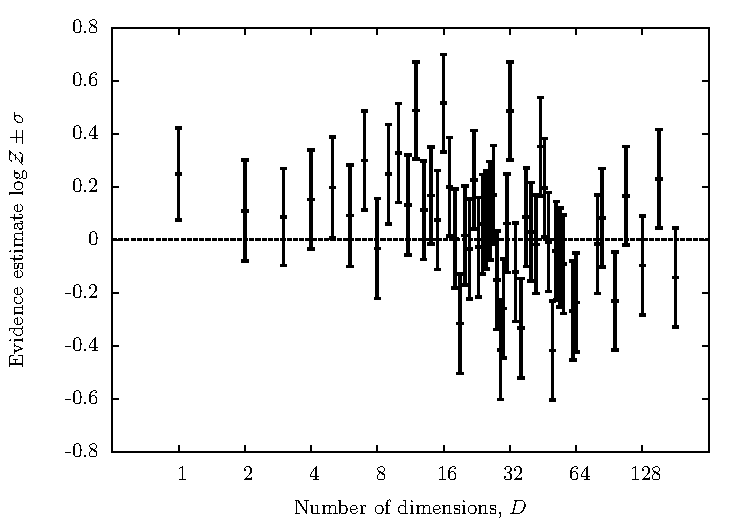
\includegraphics[width=\columnwidth]{chapters/polychord/figures/gaussian_evidences}
  \caption{%
    Evidence estimates and errors produced by \PolyChord{} for a Gaussian likelihood as a function of dimensionality. The dashed line indicates the correct analytic evidence value.\label{fig:pc:gaussian_evidences}
}
\end{figure}

\begin{figure}[tp]
  \centering
  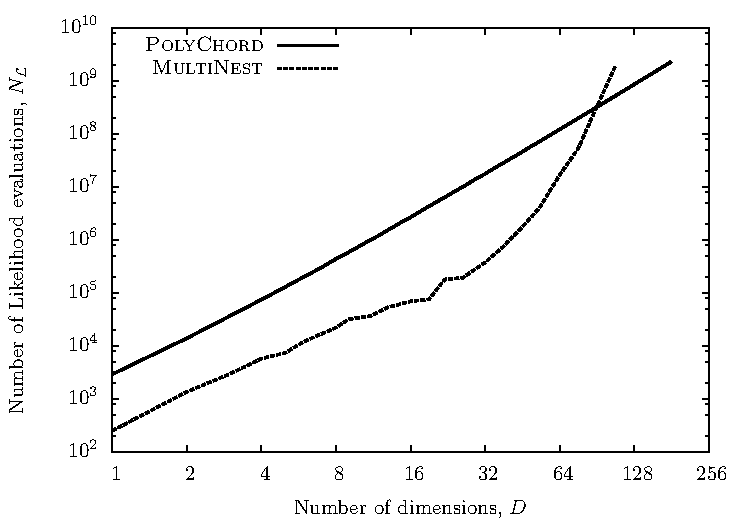
\includegraphics[width=\columnwidth]{chapters/polychord/figures/gaussian}
  \caption{Comparing \PolyChord{} with \MultiNest{} using a
  Gaussian likelihood for different dimensionalities. \PolyChord{} has at worst $\nlike\bigO{D^3}$, whereas \MultiNest{} has an exponential scaling that emerges at high dimensions.\label{fig:pc:gaussian}
}
\end{figure}

\subsection{Clustering and local evidences}
\label{sec:pc:loc_ev}
To demonstrate \PolyChord{}'s clustering capability we report its performance on a ``Twin Peaks'' and Rastrigin likelihood.

\subsubsection{Twin peaks}
\label{sec:pc:twin_peaks}
\PolyChord{} is capable of clustering posteriors in very high dimensions. We define a twin peaks likelihood as an equal mixture of two spherical Gaussians, separated by a distance of 10$\sigma$.

\PolyChord{} correctly identifies these clusters in arbitrary dimensions (tested up to $D=100$), providing that $\nlive$ and $\nrepeats$ are scaled in proportion to $D$. It calculates a global evidence that agrees with the analytic results. In addition, the local evidences correctly divide the peaks in proportion to their evidence contribution.

The results for a twin peaks likelihood are of an identical character to Figures~\ref{fig:pc:gaussian_evidences}~\&~\ref{fig:pc:gaussian}, and hence not included.

\subsubsection{Rastrigin function}
\label{sec:pc:rastrigin}

\begin{figure}[tp]
  \centering
  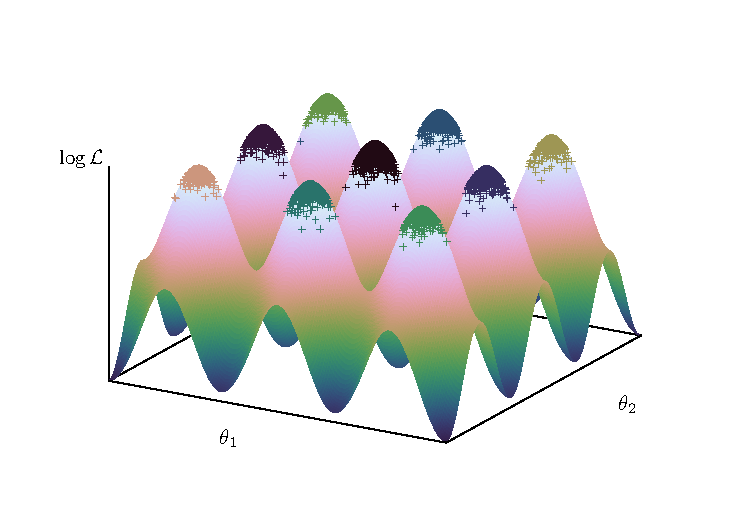
\includegraphics[width=\columnwidth]{chapters/polychord/figures/rastrigin}
  \caption{The two-dimensional Rastrigin $\log$-likelihood in the range ${[-1.5,1.5]}^2$. Within this region there are $8$ local maxima, and one global maximum at $(0,0)$. The clustered samples produced by \PolyChord{} are plotted on the $\log$-likelihood surface, with colours that indicating the separate clusters identified.\label{fig:pc:rastrigin}}
\end{figure}

\begin{figure}[tp]
  \centering
  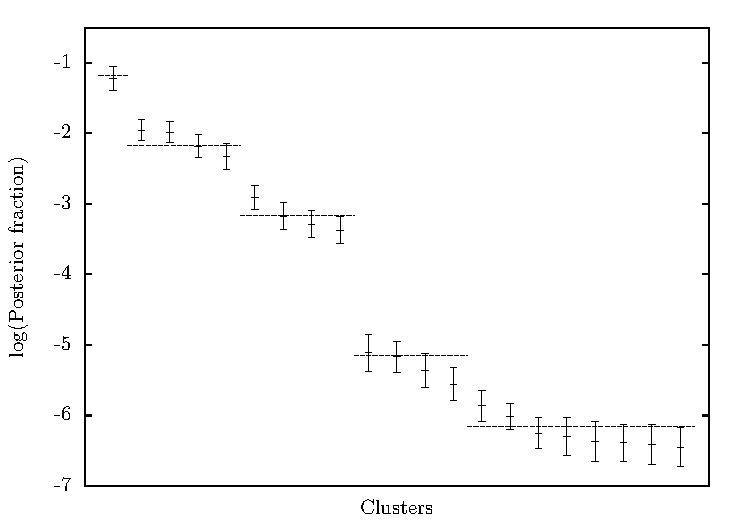
\includegraphics[width=\columnwidth]{chapters/polychord/figures/rastrigin_data}
  \caption{\PolyChord{} cluster identification for the Rastrigin function. \PolyChord{} identifies posterior modes and computes their local evidences, expressed here as a logarithmic fraction of  the total evidence in the mode. Dashed lines indicate the analytic results computed by a saddle point approximation at each of the peaks. As can be seen, \PolyChord{} reliably identifies the inner $21$ modes with increasing accuracy.\label{fig:pc:rastrigin_data}}
\end{figure}

\PolyChord{}'s clustering capacity is very effective on complicated clustering problems as well. The $n$-dimensional Rastrigin test function is defined by:
\begin{align}
  f(\theta) &= A n + \sum\limits_{i=1}^n \left[\theta_i^2 - A\cos(2 \pi \theta_i) \right],
  \label{eqn:pc:rastrigin_function}
  \\
  A&=10, \qquad \theta_i \in [-5.12,5.12]. \nonumber
\end{align}
This is the industry standard ``bunch of grapes'', the two-dimensional version of which is illustrated in Figure~\ref{fig:pc:rastrigin}.
For our purposes, we will treat~\eqref{eqn:pc:rastrigin_function} as the negative log-likelihood so that $\lik(\theta) \propto \exp[-f(\theta)]$.
This is a stereotypically hard problem to solve, as many algorithms get stuck in local maxima.



We ran \PolyChord{} on a two-dimensional Rastrigin log-likelihood  with $\nlive=1000$ and $\nrepeats=6$. With these settings, \PolyChord{} calculates accurate evidence and posterior samples (Figure~\ref{fig:pc:rastrigin}), and in addition correctly isolates and computes local evidences for the inner $21$ modes. Additional outer modes are also found, but these are combinations of lower modes due to their very low posterior fraction. Increasing the resolution parameter $\nlive$ further increases the number of modes identified.  Examples of clustered posterior samples are indicated in Figure~\ref{fig:pc:rastrigin_data}, coloured using \citepos{cubehelix} `cubehelix'.


\subsection{Rosenbrock function}
\label{sec:pc:rosenbrock}

\begin{figure}[tp]
  \centering
  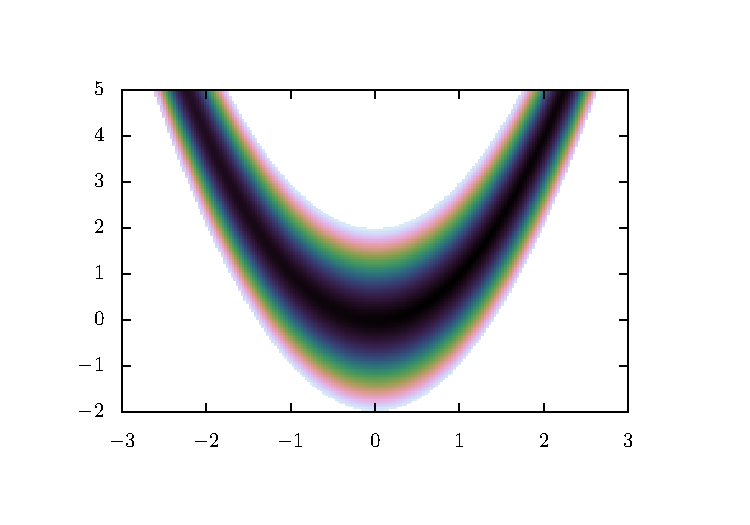
\includegraphics[width=\columnwidth]{chapters/polychord/figures/rosenbrock_analytic}
  \caption{Density plot of the two-dimensional Rosenbrock function. The function exhibits a long, thin curving degeneracy, with a global maximum at $(1,1)$.\label{fig:pc:rosenbrock_2d}}
\end{figure}

\begin{figure}[tp]
  \centering
  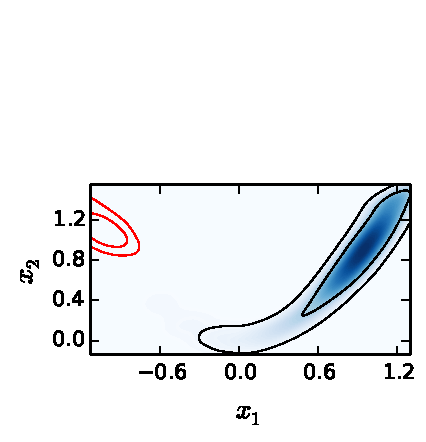
\includegraphics[width=\columnwidth]{chapters/polychord/figures/rosenbrock}
  \caption{The four-dimensional Rosenbrock posterior, with $x_3$ and $x_4$ marginalised out. \PolyChord{} correctly identifies both the local (red) and global (blue) maxima.\label{fig:pc:rosenbrock}}
\end{figure}

\PolyChord{} is also capable of navigating moderate curving degeneracies. 

The $n$-dimensional Rosenbrock function is defined by:
\begin{align}
  f(x) &= \sum\limits_{i=1}^{n-1}   {(a-x_i)}^2+ b {(x_{i+1} -x_i^2 )}^2,
    \label{eqn:pc:rosenbrock}
    \\
    a&=1,\quad b=100,\quad x_i\in[-5,5],
\end{align}
the two-dimensional version of which is plotted in Figure~\ref{fig:pc:rosenbrock_2d}. This is the industry standard ``banana'', as it exhibits an extremely long and flat curving degeneracy. We consider ${n=4}$, in which there is a global maximum at $(1,1,1,1)$ and a local maximum at $(-1,1,1,1)$. The true evidence value is $-15.1091$, and with $\nlive=1000,\nrepeats=12$, \PolyChord{} reliably finds both peaks (Figure~\ref{fig:pc:rosenbrock}) and produces a correct evidence estimation.

In higher dimensions, \PolyChord{} reliably finds the local and global maxima. The lack of an analytic evidence value for the Rosenbrock function prevents a verification of the evidence calculation.

\subsection{Gaussian shells}
\label{sec:pc:gaussian_shells}

A ``Gaussian shell'' with mean $\bmew$, radius $r$ and width $w$ is defined as:
\begin{equation}
  \log\lik_\sshell(\bxx|\bmew,r,w) = A - \frac{{\left(\left|\bxx - \bmew\right|- r\right)}^2}{2w^2},
  \label{eqn:pc:gaussian_shell}
\end{equation}
where $A$ is a normalisation constant that may be calculated using a saddle point approximation.
This likelihood is centered on some mean vector $\bmew$, and has a radial Gaussian profile with width $w$ at distance $r$ from this centre. This radial profile is then revolved around $\bmew$ to create a spherical shell-like likelihood. A two-dimensional version of this likelihood is indicated in Figure~\ref{fig:pc:gaussian_shell}.

This distribution may be representative of likelihoods that one may encounter in beyond-the-Standard-Model paradigms in particle physics. In such models, the majority of the posterior mass lies in thin sheets or hypersurfaces through the parameter space.

Running \PolyChord{} on a $100$-dimensional Gaussian shell with $\nlive=1000$, $\nrepeats=200$ yields consistent evidences and posteriors, shown in Figure~\ref{fig:pc:gaussian_shell_posterior}. 
                                                                  
Given that this problem is quoted as being ``optimally difficult'' \citep{MultiNest2}, the ease with which \PolyChord{} tackles this problem in high dimensions is worth explanation. In the two-dimensional case, it is clear that the posterior mass is concentrated in a very thin, curving region of the parameter space. However, as the dimensionality is increased, more and more of the $n$-sphere's volume is concentrated at the edge, and the thin characteristic of the degeneracy is lost. 

This may mean that the Gaussian shell is not a good proxy for a high-dimensional curving degeneracy. However, it could equally suggest that curving degeneracies become easier to navigate in higher dimensions. We can certainly conclude that a particle physics model with a proliferation of phases would be easier to navigate than one with a smaller number of phases.


\begin{figure}[tp]
  \centering
  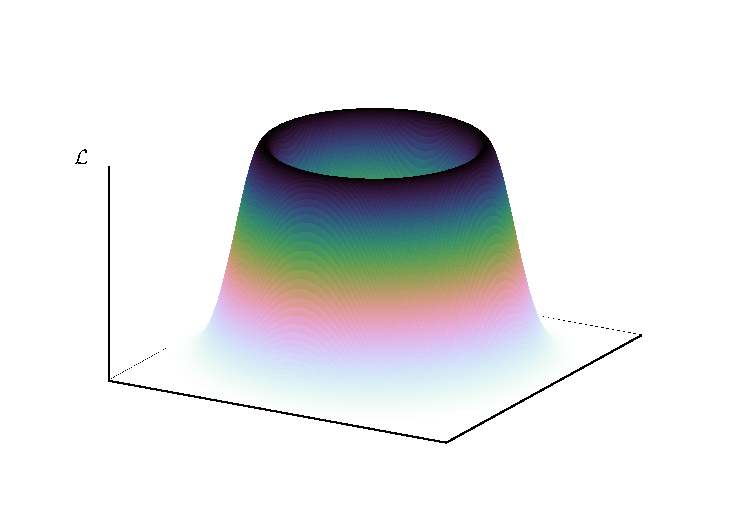
\includegraphics[width=\columnwidth]{chapters/polychord/figures/gaussian_shell}
  \caption{The two-dimensional Gaussian shell likelihood.\label{fig:pc:gaussian_shell}}
\end{figure}

\begin{figure}[tp]
  \centering
  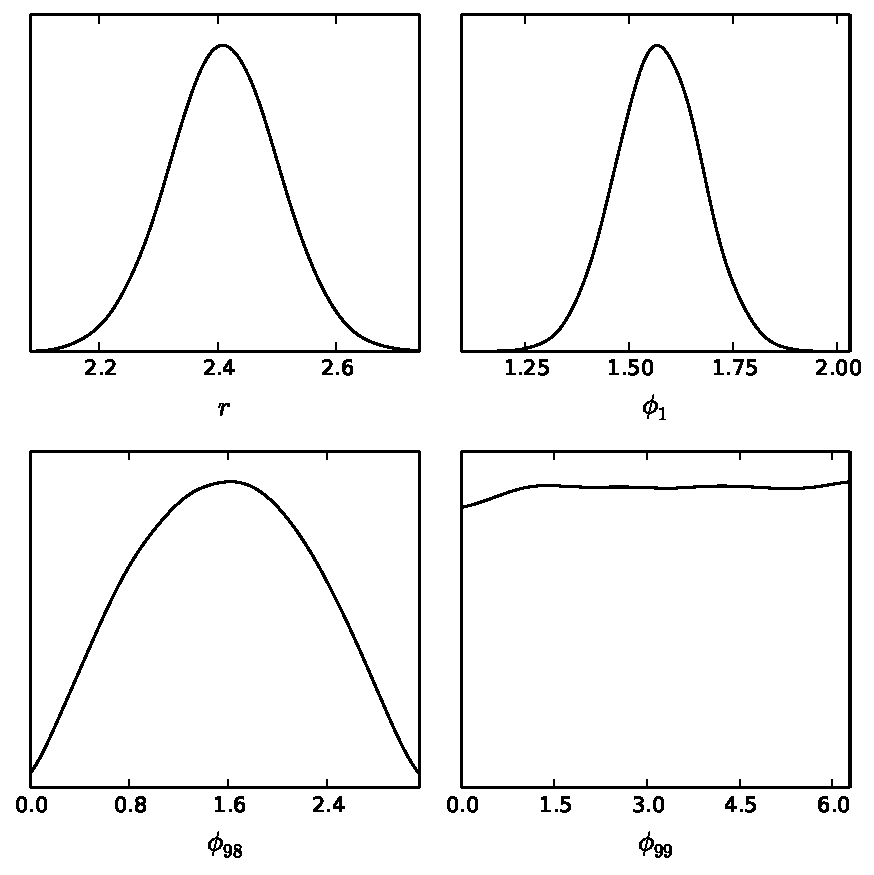
\includegraphics[width=\columnwidth]{chapters/polychord/figures/gaussian_shell_posterior}
  \caption{Posteriors produced by \PolyChord{} for a $n=100$-dimensional Gaussian shell, with width $w=0.1$, radius $r=2$, and center $\bmew=\bzero$. 
  Plotting the marginalised posteriors for the Cartesian sampling parameters ${\{x_1,\ldots,x_n\}}$ yields Gaussian distributions centered on the origin. To see the effectiveness of the sampler it is better to plot the sampling parameters in terms of $n$-dimensional spherical polar co\"{o}rdinates ${\{r,\phi_1,\ldots,\phi_{n-1}\}}$. Note that the polar co\"{o}rdinates are {\em derived parameters}, and that the sampling space still has the strong Gaussian shell degeneracy.
  In this case we can see that the radial co\"{o}rdinate has a Gaussian profile centered on $r_0 = r\times\frac{1}{2} {\left(1 + \sqrt{1 +  4 (n-1) {\left({w}/{r}\right)}^2}\right) }$ with width $w_0 = w{(1+(n-1){(w/r_0)}^2)}^{-1/2}$. 
  The azimuthal co\"{o}rdinate $\phi_{n-1}$ has a uniform posterior, and the other angular co\"{o}rdinates $\{\phi_i\}$ have posteriors defined by $\Prob{\phi_i } \propto {{\left(\sin\phi_i\right)}^{n-i-1}}$.
\label{fig:pc:gaussian_shell_posterior}
}
\end{figure}


\subsubsection{Twin Gaussian shells}
We finish our toy problems by combining the difficulties of multimodality (Section~\ref{sec:pc:loc_ev}) and degeneracy, by mixing two twin Gaussian shells together:
\begin{equation}
  \lik(\bxx) \propto \lik_\sshell(\bxx|\bmew_1,r,w) + \lik_\sshell(\bxx|\bmew_2,r,w).
  \label{eqn:pc:gaussian_shells}
\end{equation}
We choose $r=2$, $w=0.1$, and $\mu_1$ and $\mu_2$ are separated by $7$ units. With $\nlive=10\ndims$ and $\nrepeats=2\ndims$, \PolyChord{} successfully computes the local and global posteriors and evidences up to $D=100$, and reliably identifies the two modes. The comparison of run times with \MultiNest{} recovers a similar pattern to Figure~\ref{fig:pc:gaussian}, although in our experience, the \MultiNest{} parameters require some tuning to ensure that evidences are calculated correctly when $\ndims>30$.


\subsection{\CosmoChord}
\label{sec:pc:cosmochord}

\begin{figure}[tp]
  \centering
  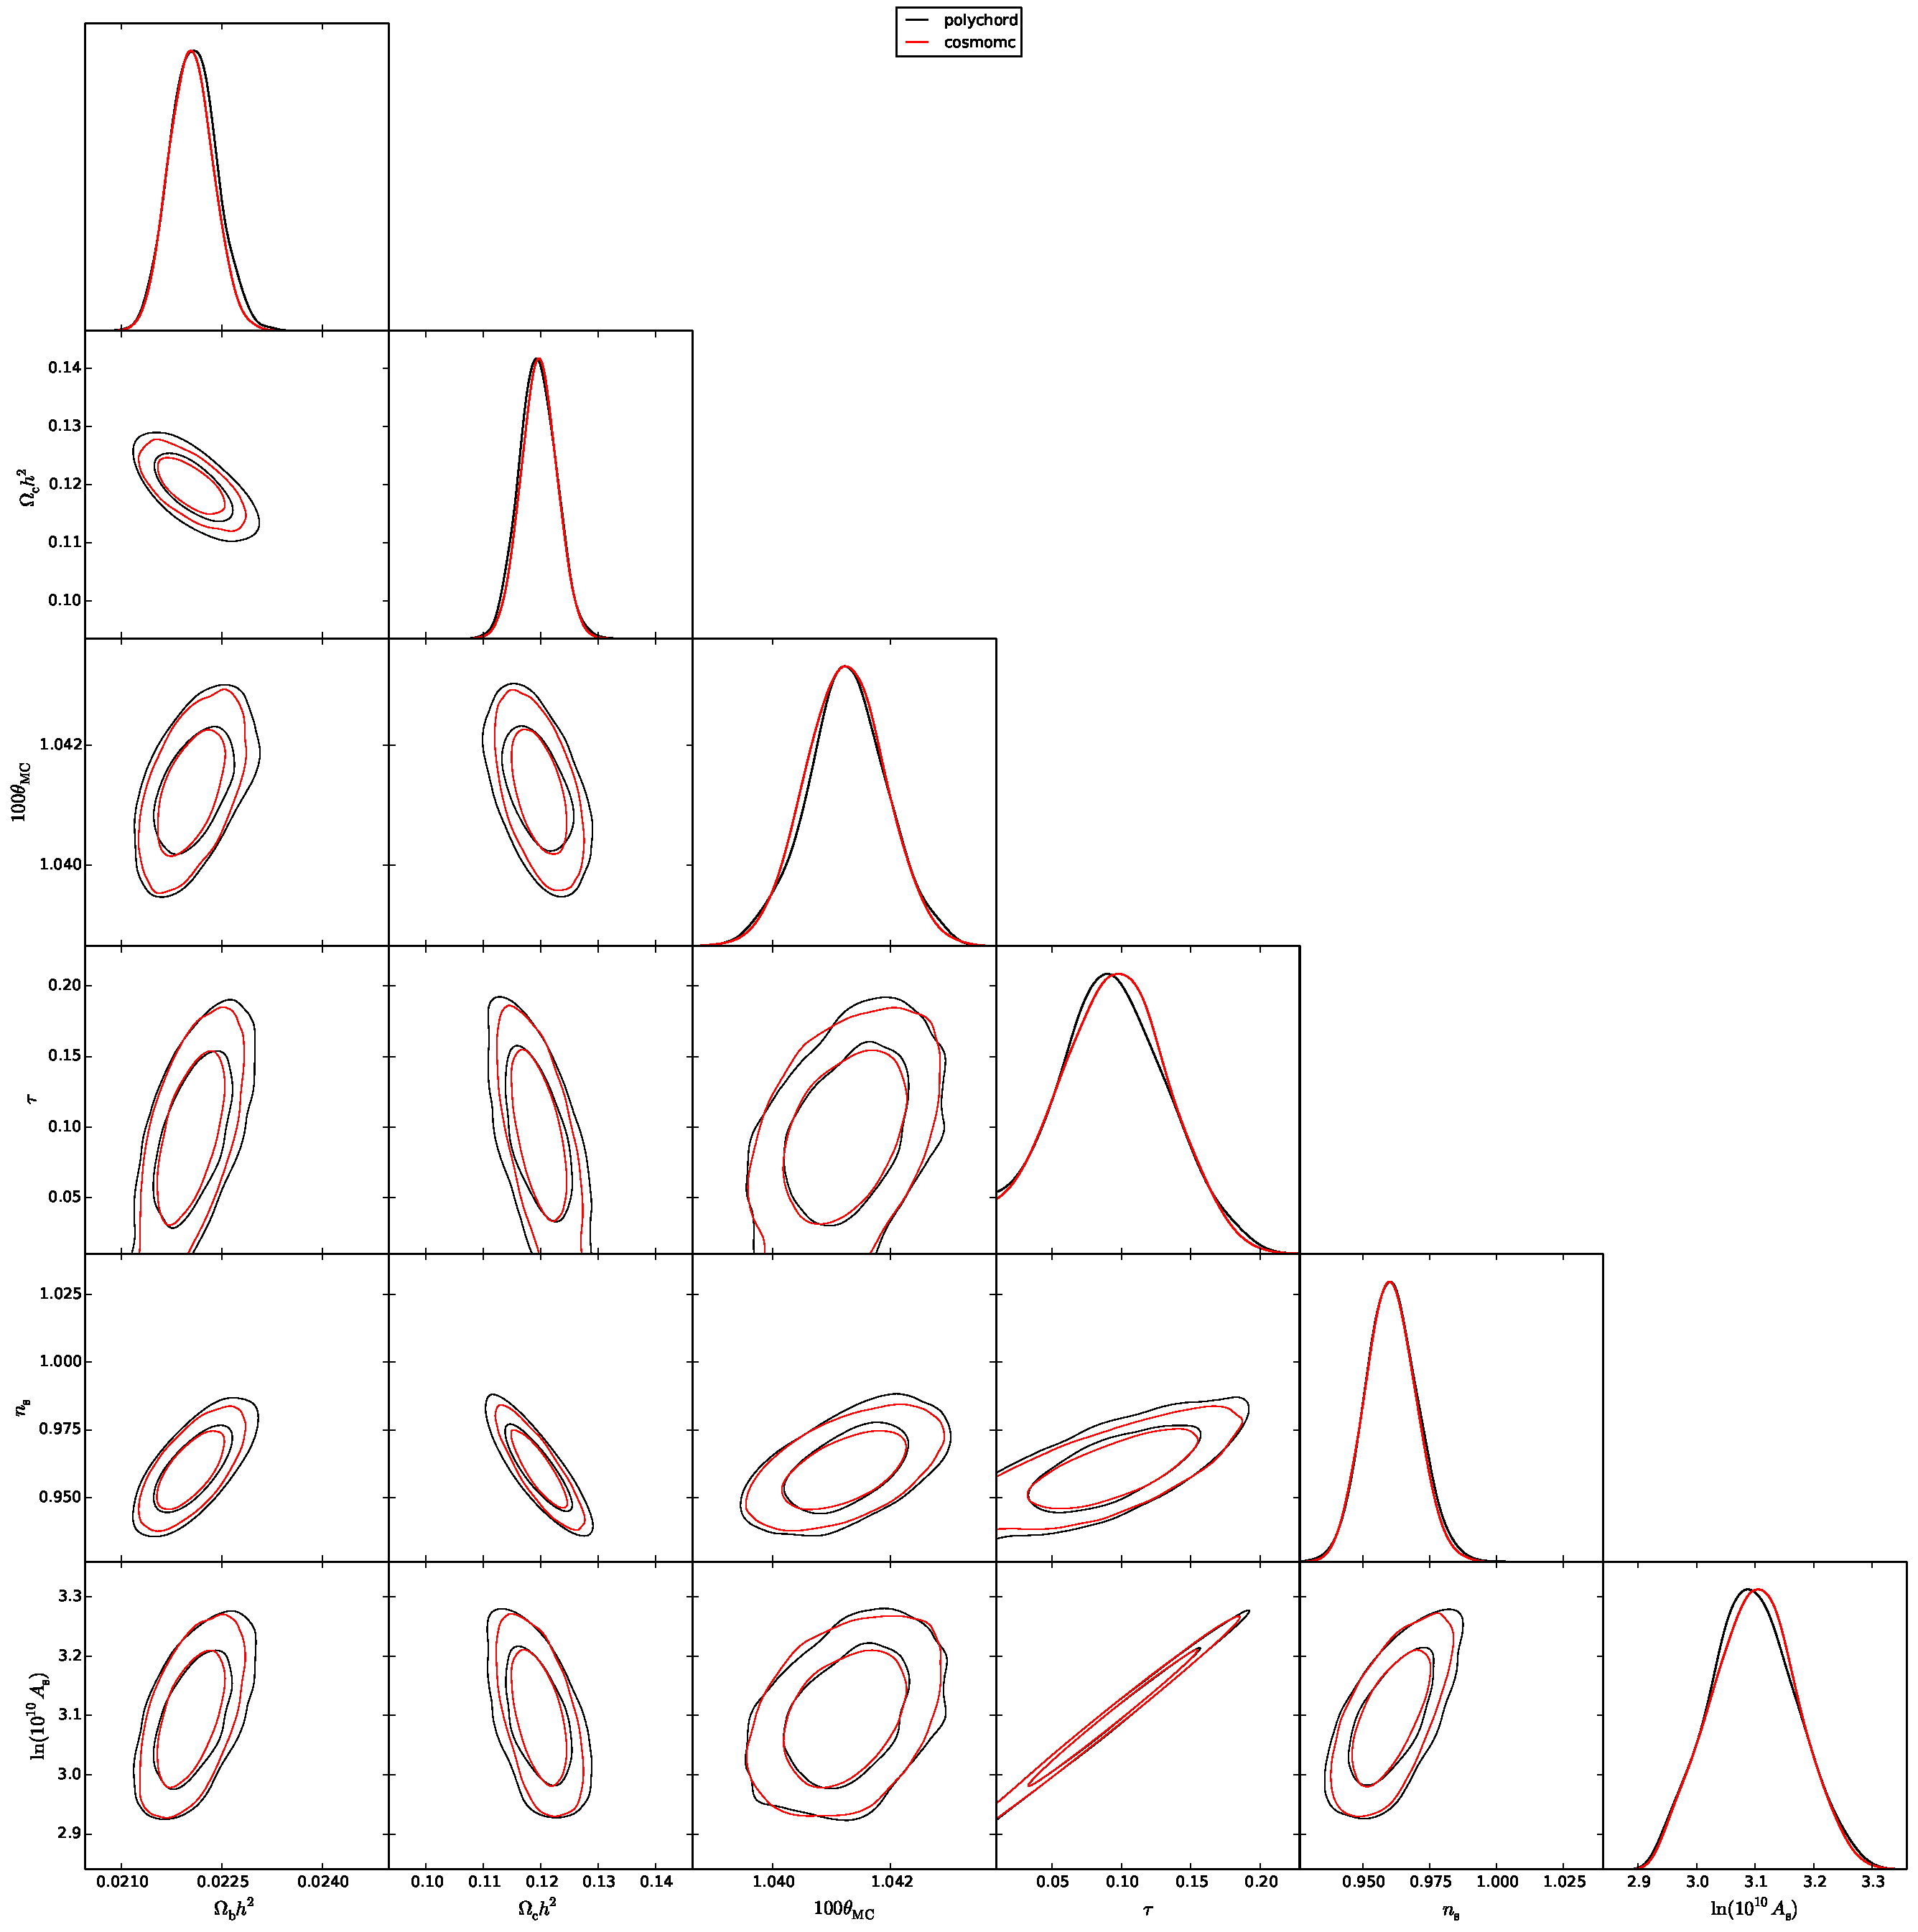
\includegraphics[width=\textwidth]{chapters/polychord/figures/cosmochord}
  \caption{\CosmoChord{} (red) vs.\ \CosmoMC{} (black). We use the 2013 {\texttt CAMSPEC}+{\texttt commander} likelihoods with a standard six-parameter $\Lambda$CDM cosmology, varying all 14 nuisance parameters.  We compare the $1$ and $2$-dimensional marginalised posteriors of the $6$ $\Lambda$CDM parameters. \CosmoChord{} is in close agreement with the posteriors produced by \CosmoMC{}, recovering the correct mean values of and degeneracies between the parameters. The slight deviations between the red and black curves are sampling noise.\label{fig:pc:cosmochord}}
\end{figure}

An additional strength of \PolyChord{} lies in its ability to exploit a fast-slow hierarchy common in many cosmological applications. 

As an example, we consider the likelihoods provided by \CAMB{}~\citep{CAMB} and \CosmoMC{}~\citep{cosmomc}. In Boltzmann codes such as \CAMB{}, parameters controlling the primordial power spectrum (such as $n_s$ and $A_s$) do not require recalculation of transfer functions. These parameters are termed ``semi-slow''. In addition, modern Planck likelihoods~\citep{Planck2013Like} have nuisance parameters associated with the foregrounds. These may be varied without recalculation of the cosmological background. These parameters are hence termed ``fast''. \CosmoMC{}~\citep{cosmomc} implements this hierarchy of speeds in its likelihood calculation.

We have successfully implemented \PolyChord{} within \CosmoMC{}, and term the result \CosmoChord{}.  The traditional Metropolis-Hastings algorithm is replaced with nested sampling. This implementation is available to download from the link at the end of the paper.

The exploitation of fast-slow parameters means that \CosmoChord{} vastly outperforms \MultiNest{} when running with modern Planck likelihoods. 

\CosmoMC{} by default uses a Metropolis-Hastings sampler. If this has a well-tuned proposal distribution (e.g.\ if one is performing importance sampling from an already well-characterised likelihood), then \PolyChord{} is $2$--$4$ times slower than the traditional \CosmoMC{}. If proposal matrices are unavailable (e.g.\ in the case that one is examining an entirely new model) then \CosmoChord{}'s run time is competitive with the native \CosmoMC{} sampler. This is a good example of the self-tuning capacity of \PolyChord{}, since it only requires two tuning parameters, as opposed to $\bigO{D^2}$.

\CosmoChord{} produces parameter estimations consistent with \CosmoMC{} (Figure~\ref{fig:pc:cosmochord}).
It has been implemented effectively in multiple cosmological applications in the latest Planck paper describing constraints on inflation~\citep{planck2015-a24}, including application to a $37$-parameter reconstruction problem ($4$ slow, $19$ semi-slow, $14$ fast). 
In addition, \PolyChord{} is an integral component of the \ModeChord{} code, a combination of \CosmoChord{} and \ModeCode{} \citep{ModeChord1,ModeChord2,ModeChord3}, which is available at \url{http://modecode.org/}.

\section{Conclusions}
\label{sec:pc:conclusions}
We have introduced \PolyChord{}, a novel nested sampling algorithm tailored for high-dimensional parameter spaces. It is able to fully exploit a hierarchy of parameter speeds such as is found in \CosmoMC{} and \CAMB{}. It utilises slice sampling at each iteration to sample within the hard likelihood constraint of nested sampling. It can identify and evolve separate modes of a posterior semi-independently and is parallelised using \openMPI{}.












\section*{Download Link}
PolyChord is available for download from:\\ \url{http://ccpforge.cse.rl.ac.uk/gf/project/polychord/}

\cleardoublepage{}
